%  !TeX  root  =  user_guide.tex

\section{Getting Started}\label{label_getstarted}

% when the revision of a section has been finalized, 
% comment out the following line:
% \updatedisclaimer

This chapter gives a quick overview of installing \qg, some sample 
data from the \qg web page and running a first and simple session 
visualizing raster and vector layers.

\section{Installation}\label{label_installation}
\index{installation}

Installation of \qg is very simple. Standard installer packages are
available for MS Windows and Mac OS X. For many flavors of GNU/Linux binary
packages (rpm and deb) or software repositories to add to your installation
manager are provided. Get the latest information on binary packages at the
\qg website at \url{http://qgis.osgeo.org/download/}.

\minisec{Installation from source}

If you need to build \qg from source, please refer to the coding and
compiling guide available at \url{http://qgis.osgeo.org/documentation/}. 
The installation instructions are also distributed with the \qg source
code.

\minisec{Installation on external media}

QGIS allows to define a --configpath option that overrides the default path 
(e.g. ~/.qgis under Linux) for user configuration and forces QSettings to use 
this directory, too. This allows users to e.g. carry a QGIS installation on a 
flash drive together with all plugins and settings. 

\section{Sample Data}\label{label_sampledata}
\index{data!sample} 

The user guide contains examples based on the \qg sample dataset. 

\win The Windows installer has an option to download the \qg sample dataset.
If checked, the data will be downloaded to your \filename{My Documents}
folder and placed in a folder called \filename{GIS Database}. 
You may use Windows Explorer to move this folder to any convenient location.
If you did not select the checkbox to install the sample dataset
during the initial \qg installation, you can either
\begin{itemize}[label=--]
\item use GIS data that you already have;
\item download the sample data from the qgis website at \url{http://qgis.osgeo.org/download}; or
\item uninstall \qg and reinstall with the data download option checked, only if 
the above solutions are unsuccessful.
\end{itemize}

\nix \osx For GNU/Linux and Mac OSX there are not yet dataset installation
packages available as rpm, deb or dmg. To use the sample dataset download the
file \filename{\qg\_sample\_data} as ZIP or TAR archive from
\url{http://download.osgeo.org/qgis/data/} and unzip or untar the archive on
your system. The Alaska dataset includes all GIS data that are used as
examples and screenshots in the user guide, and also includes a small GRASS
database. The projection for the qgis sample dataset is Alaska Albers Equal
Area with unit feet. The EPSG code is 2964.

\begin{verbatim}
PROJCS["Albers Equal Area",
    GEOGCS["NAD27",
        DATUM["North_American_Datum_1927",
            SPHEROID["Clarke 1866",6378206.4,294.978698213898,
                AUTHORITY["EPSG","7008"]],
            TOWGS84[-3,142,183,0,0,0,0],
            AUTHORITY["EPSG","6267"]],
        PRIMEM["Greenwich",0,
            AUTHORITY["EPSG","8901"]],
        UNIT["degree",0.0174532925199433,
            AUTHORITY["EPSG","9108"]],
        AUTHORITY["EPSG","4267"]],
    PROJECTION["Albers_Conic_Equal_Area"],
    PARAMETER["standard_parallel_1",55],
    PARAMETER["standard_parallel_2",65],
    PARAMETER["latitude_of_center",50],
    PARAMETER["longitude_of_center",-154],
    PARAMETER["false_easting",0],
    PARAMETER["false_northing",0],
    UNIT["us_survey_feet",0.3048006096012192]]
\end{verbatim}

If you intend to use \qg as graphical frontend for GRASS, you can find a
selection of sample locations (e.g. Spearfish or South Dakota) at the
official GRASS GIS website \\
\url{http://grass.osgeo.org/download/data.php}. 

\section{Sample Session}\label{samplesession}

Now that you have \qg installed and a sample dataset available, we would 
like to demonstrate a short and simple \qg sample session. We will visualize 
a raster and a vector layer. We will use the landcover raster 
layer \filename{\qg\_sample\_data/raster/landcover.img} and the lakes 
vector layer \filename{\qg\_sample\_data/gml/lakes.gml}.

\minisec{start \qg}

\begin{itemize}[label=--]
\item \nix{Start \qg by typing: \usertext{\qg} at a command prompt, or
if using precompiled binary, using the Applications menu.}
\item \win{Start \qg using the Start menu or desktop shortcut, 
or double click on a \qg project file.}
\item \osx{Double click the icon in your Applications folder.}
\end{itemize} 

\begin{figure}[ht]
   \centering 
   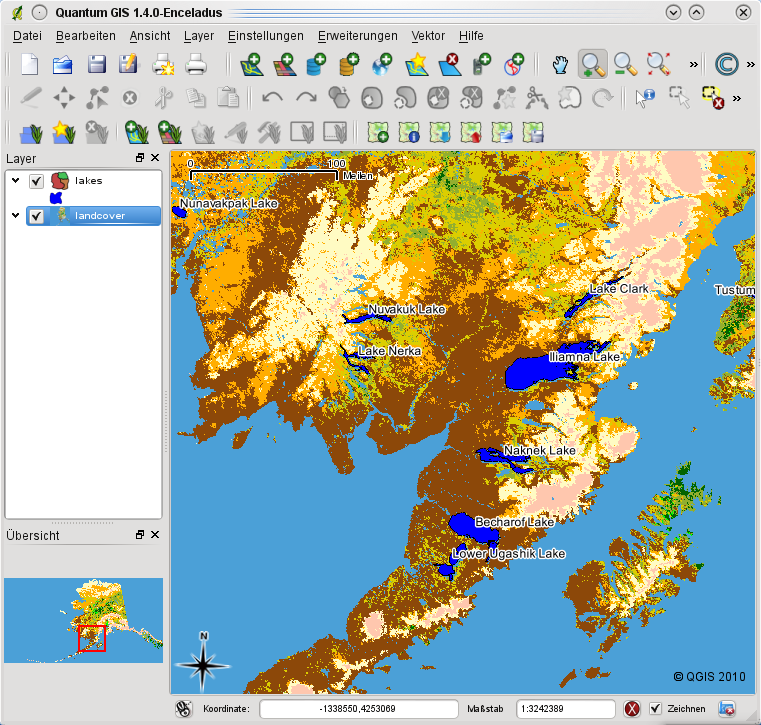
\includegraphics[clip=true, width=12cm]{simple_session}
   \caption{A Simple \qg Session \nixcaption}\label{fig:simple_session}
\end{figure}

\minisec{Load raster and vector layers from the sample dataset}

{\setlength{\baselineskip}{1.3\baselineskip}
\begin{enumerate}[itemsep=2pt]
\item Click on the \toolbtntwo{mActionAddRasterLayer}{Load Raster} icon.
\item Browse to the folder \filename{\qg\_sample\_data/raster/}, select 
the ERDAS Img file \filename{landcover.img} and click \button{Open}.
\item If the file is not listed, check if the Filetype combobox at the
bottom of the dialog is set on the right type, in this case "Erdas Imagine
Images (*.img, *.IMG)"
\item Now click on the \toolbtntwo{mActionAddOgrLayer}{Load Vector} icon. 
\item \radiobuttonon{'File'} should be selected as Source Type in the new
\dialog{Add Vector Layer} dialog. Now click \button{Browse} to select the
vector layer.
\item Browse to the folder \filename{\qg\_sample\_data/gml/}, select "GML"
from the filetype combobox, then select the GML file \filename{lakes.gml} 
and click \button{Open}, then in Add Vector dialog click \button{OK}.
\item Zoom in a bit to your favorite area with some lakes.
\item Double click the \filename{lakes} layer in the map legend to open the 
\dialog{Layer Properties} dialog.
\item Click on the \tab{Symbology} tab and select a blue as fill color.
\item Click on the \tab{Labels} tab and check the \checkbox{Display labels} 
checkbox to enable labeling. Choose NAMES field as Field containing label.
\item To improve readability of labels, you can add a white buffer around them,
by clicking ``Buffer'' in the list on the left, checking \checkbox{Buffer
labels?} and choosing 3 as buffer size.
\item Click \button{Apply}, check if the result looks good and finally
click \button{OK}.
\end{enumerate} 
\par}
You can see how easy it is to visualize raster and vector layers in 
\qg. Let's move on to the sections that follow to learn more about the 
available functionality, features and settings and how to use them.

\FloatBarrier
